\projecthead{01}{PsiSat}{A 1U gamma-ray burst nanosatellite}{July 2026 - present}
\textit{Design study / proposal}
\par\medskip A student CubeSat proposal to detect short flashes of high-energy light from orbit, with a compact aluminum shell and six planned electronics layers.
\par\smallskip {\small\color{muted} Tools: Fusion 360, PCB design, detector integration}
\medskip
\noindent
\begin{minipage}[t]{.48\linewidth}\centering\vspace{0pt}
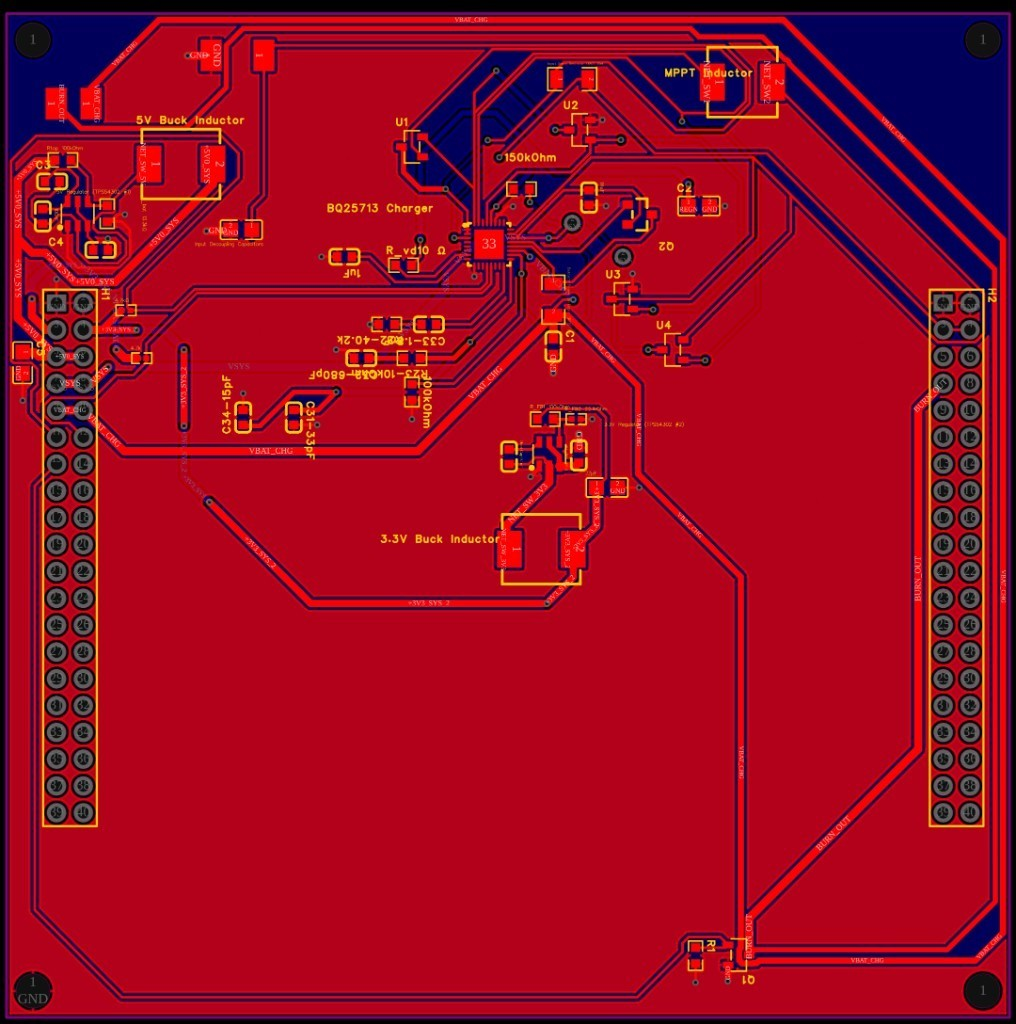
\includegraphics[width=\linewidth,height=2.5in,keepaspectratio]{images/psisat/power-layout.jpg}
\par\smallskip{\footnotesize\color{muted} Stage 4: power board layout.}\end{minipage}\hfill
\begin{minipage}[t]{.48\linewidth}\centering\vspace{0pt}
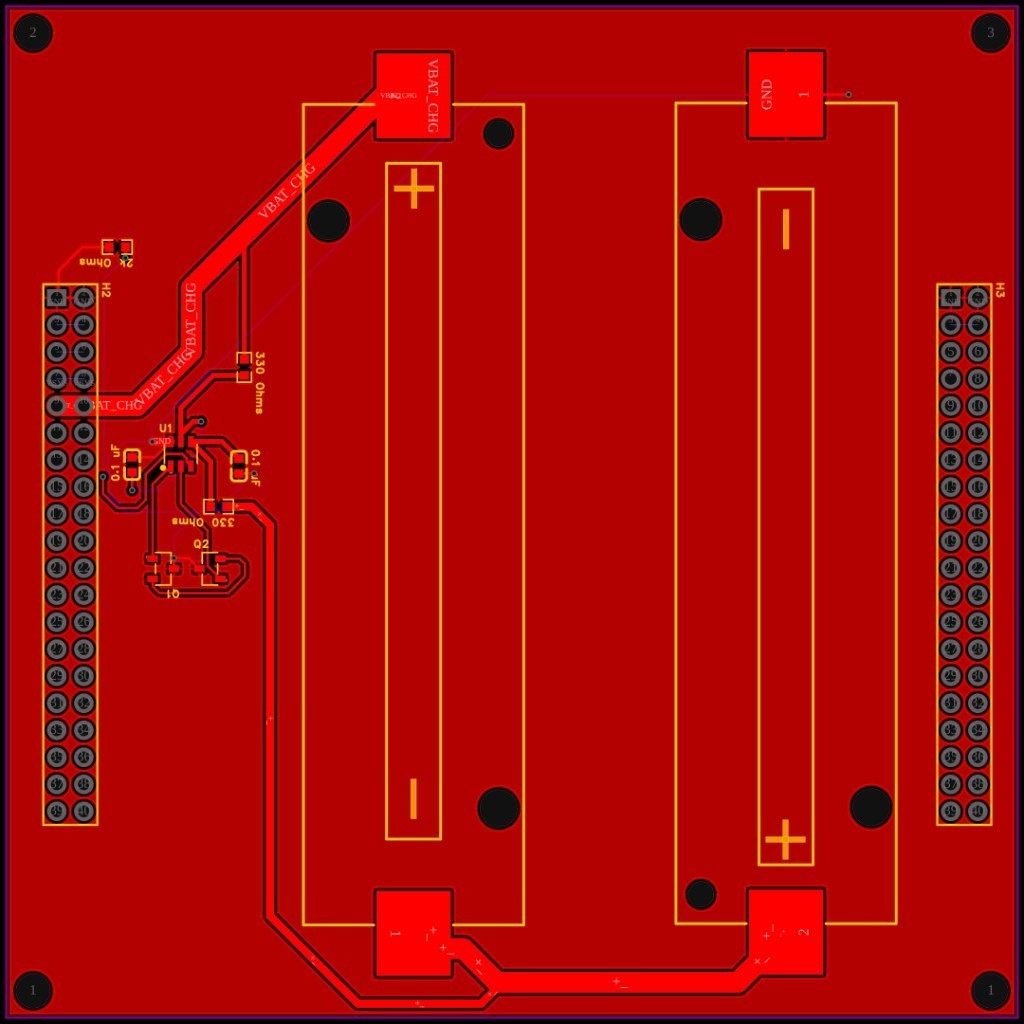
\includegraphics[width=\linewidth,height=2.5in,keepaspectratio]{images/psisat/battery-layout.jpg}
\par\smallskip{\footnotesize\color{muted} Stage 5: battery board layout.}\end{minipage}\hfill
\par\medskip
\subsection*{Purpose}
A scintillator converts incoming gamma rays into light near 550 nm. A sensor reads each flash and a small computer records its timing.
\subsection*{My contribution}
I started the project, recruited the team, and wrote the NASA CubeSat Launch Initiative proposal. The shell is modeled in Fusion 360. Jackson Boyle and Christian Tumanda are also on the proposal.
\subsection*{Packaging \& status}
The target envelope is about 10 x 10 x 11 cm, with mass below 1.33 kg. Six electronics layers are planned. Stage 4 is the power board and Stage 5 holds the batteries; four other boards remain in design. PsiSat has not launched.
\medskip\href{https://github.com/leosgxsbu/Psi_Sat-1U-CubeSat-}{View project repository}